%% Richard Wen
%% rwen@ryerson.ca


% *** APPENDICES ***


\appendix

\section{Literature Review Methods}  \label{appendix:literature-review-methods}

\subsection{Digital Library Selection} \label{appendix:digital-library-selection}

The papers for the literature review were found with the search engines available in the Association for Computing Machinery (ACM) \cite{ACM:2017} and Institute of Electrical and Electronics Engineers (IEEE) Xplore digital libraries \cite{IEEE:2017}. A search for the top journals in computer science by journal impact factor \cite{Garfield:2006b} was done using the InCites journal citation reports web tool \cite{Clarivate:2017a}. A majority of ACM and IEEE journals were found to be in the first quartile of journal impact factor values for the computer science category. A visualization of the top 25 journals in computer science by journal impact factor in 2016 is shown in Figure \ref{figure:incites_top25jifcs}.

\begin{figure}[!t]
	\centering
	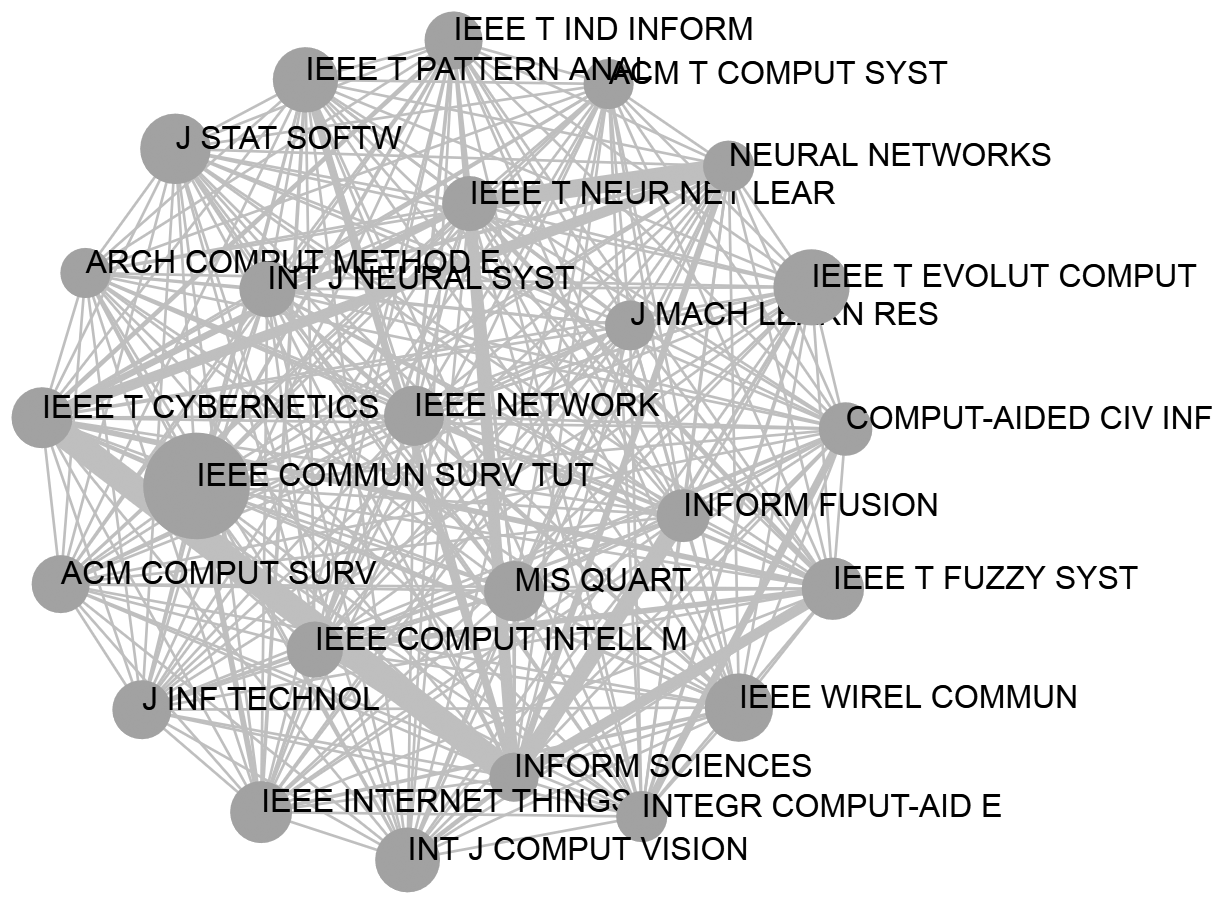
\includegraphics[width=2.5in]{incites_top25jifcs}
	\caption{\textbf{Top 25 Computer Science Journals by Journal Impact Factor from InCites Journal Citation Report in 2016.} Gray circles represent the Journal Impact Factor, where higher Journal Impact Factor values are represented by larger sizes. Connected lines represent the citation relationships between each journal, where thicker lines mean stronger relationships.}
	\label{figure:incites_top25jifcs}
\end{figure}

The search for the top 25 computer science journals was based on the Journal Impact Factor (JIF) \cite{Garfield:2006b} measure, and was done using the InCites Journal Citation Reports (JCR) web tool \cite{Clarivate:2017a}. The search used the following options available on InCites:

\begin{itemize}
  \item \textbf{Categories}:
	\begin{itemize}
		\item COMPUTER SCIENCE, ARTIFICIAL INTELLIGENCE
		\item COMPUTER SCIENCE, CYBERNETICS
		\item COMPUTER SCIENCE, HARDWARE \& ARCHITECTURE
		\item COMPUTER SCIENCE, INFORMATION SYSTEMS
		\item COMPUTER SCIENCE, INTERDISCIPLINARY APPLICATIONS
		\item COMPUTER SCIENCE, SOFTWARE ENGINEERING
		\item COMPUTER SCIENCE, THEORY \& METHODS
	\end{itemize}
  \item \textbf{JCR Year}: 2016
  \item \textbf{Edition}: Science Citation Index Expanded (SCIE) \cite{Garfield:2006a} and Social Sciences Citation Index (SSCI) \cite{Klein:2004}
  \item \textbf{Category Schema}: Web of Science \cite{Clarivate:2017b}
  \item \textbf{JIF Quartile}: Quarter 1 (Q1)
\end{itemize}

\subsection{Automatic Search Queries} \label{appendix:automatic-search-queries}

Potential papers were found using search engine queries in the ACM \cite{ACM:2017} and IEEE Xplore \cite{IEEE:2017} digital libraries identified in Appendix \ref{appendix:digital-library-selection}. Search queries were modified from the defaults and sorted by relevance. Each search query was defined to filter for potential papers with the following requirements:

\begin{enumerate}[label=(\alph*)]
	\item \textbf{Publication}: Published in ACM or IEEE
	\item \textbf{Year}: Published from 2012 to December 2, 2017
	\item \textbf{Keywords}: Contains the keywords \textit{"real time"} and \textit{"social media"} in the paper title, and \textit{"prediction"}, \textit{"predict"}, \textit{"detection"}, or \textit{"detect"} anywhere in the text
\end{enumerate}

The query syntax in the ACM digital library was accessed through the advanced search page by clicking \textit{"show query syntax"}. The \textit{"+"} symbol includes each keyword in the title. \textit{"gte"} and \textit{"lte"} represent \textit{"greater than or equal to"} and \textit{"less than or equal to"} respectively. The publication date query syntax must be manually generated using the web interface. The full advanced query syntax used for the ACM digital library to return potential papers is shown below:

\lstinputlisting{data/acm_querysyntax.txt}

The command search in the IEEE Xplore digital library was accessed through the advanced search page by clicking \textit{"command search"}. Refinements were manually applied using the web interface to filter command search results for the years 2012 to 2017 and to search in \textit{"Full Text \& Metadata"}. The command search used for the IEEE Xplore digital library to return potential papers is shown below:

\lstinputlisting{data/ieeexplore_commandsearch.txt}

\subsection{Manual Selection Criteria} \label{appendix:manual-selection-criteria}

The potential papers from Appendix \ref{appendix:automatic-search-queries} were further filtered with the abstracts and paper length. The abstracts were inspected for relevancy to the topic: \textit{"real-time geosocial media event detection and prediction"}. This included mentions of methods that deal with detecting or predicting real-world events in real-time using geosocial media data. After inspections of the abstract, each paper was further evaluated for practicality by searching for mentions of event prediction or detection applications, benchmarks, and experiments in the results sections. The manual selection criteria sought to find papers with the following characteristics:

\begin{enumerate}[label=(\alph*)]
	\item \textbf{Detailed}: Paper contained sufficient details and explanations to obtain a general understanding of the methods and results
	\item \textbf{Relevant}: Paper had mentions of real-time geosocial media event detection or prediction
	\item \textbf{Practical}: Paper had conducted experiments, benchmarks, or applications using described event detection or prediction methods
\end{enumerate}

\subsection{Review Procedure} \label{appendix:review-procedure}

A literature review of the papers selected using the methods in Appendix \ref{appendix:manual-selection-criteria} was done with the following procedure:

\begin{enumerate}
	\item \textbf{Identify} methods used for real-time geosocial media event detection or prediction
	\item \textbf{Summarize} methods in (1)
	\item \textbf{Summarize} applications and results for the methods in (1)
	\item \textbf{Discuss} limitations, possible improvements, and future directions relative to the summaries from (2) and (3)
\end{enumerate}

